\chapter{Education}

\section*{Number of children supported to gain a decent education.}
% make sure numbers and header don't appear

\thispagestyle{empty}


\section{Results}
Between 2015 and 2020 DFID supported at least \textbf{15.6 million} children to gain a decent education. %

This is the equivalent number of children fully educated by DFID. %
All DFID education programmes include a focus on quality of education, so all children counted are being helped to gain a decent education. %

\begin{figure}[htbp]
  \centering
  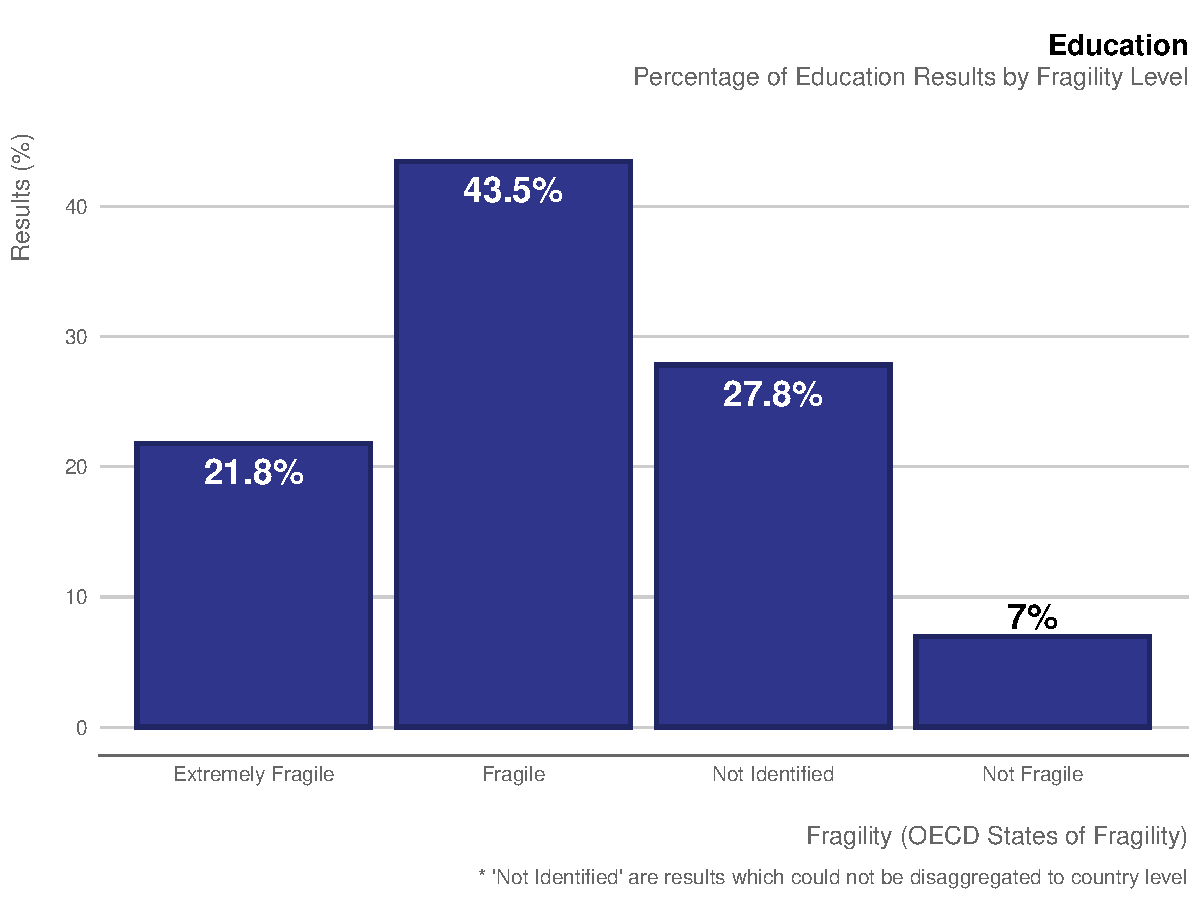
\includegraphics[width=0.8\textwidth]{../figs/education_fragility_plot} \hfill
  \caption{Percentage of Education results by fragility level.}
  \label{fig:edu_fragility_plot}
\end{figure}

From 2015 to 2020, the largest number of children supported by DFID education programmes were in Africa, with 5.6 million children supported (including 1.2 million in Ethiopia). %
DFID supported 5.3 million children in Asia (including 1.8 million in Bangladesh, and 2.1 million in Pakistan), and 0.8 million children in the Middle East. %
A further 4.6 million children were supported via centrally managed programmes and multilateral organisations. %

\begin{figure}[htbp]
	\centering
	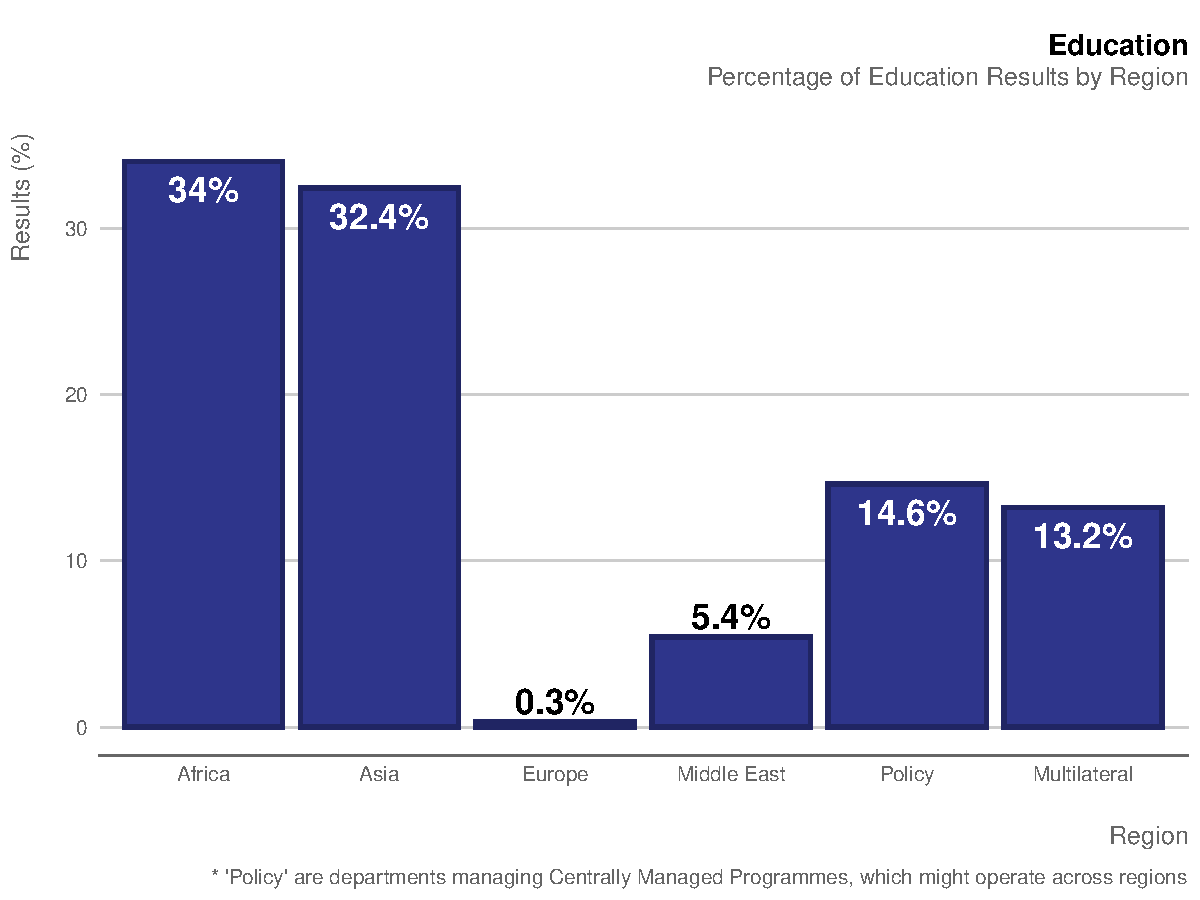
\includegraphics[width=0.8\textwidth]{../figs/education_region_plot} \hfill
	\caption{Percentage of Education results by region.}
	\label{fig:edu_region_plot}
\end{figure}

DFID uses the OECD list of fragile states, which is used to ensure our resources are focussed on fragile states. %
Most of the children supported by DFID's education programmes live in fragile states (10.8 million children), including 3.6 million living in extremely fragile states. %

Of the results that can currently be disaggregated by gender from 2015 to 2020 DFID education programs supported 8.1 million girls (over 50\% of the results). %
DFID is continuously working with our partners to improve collection of disaggregated data.
Over 95\% of our results are disaggregated by gender in part due to improvments in calculating children reached by multilateral organisations. %


\section{Context}

Education has wide ranging social, health and economic benefits. %
The latest evidence suggests:
\begin{itemize}
\item Each additional year of schooling typically results in a 10\% boost in earnings, with larger increases for women.\footnote{Montenegro, C. and Patrinos, H. (2014). Comparable Estimates of Returns to Schooling Around the World. Policy Research Working Paper. Washington DC: World Bank. Available from: \href{http://documents.worldbank.org/curated/en/830831468147839247/pdf/WPS7020.pdf}{http://documents.worldbank.org/curated/en/830831468147839247/pdf/WPS7020.pdf} [Accessed 26 January 2018]}
\item Educated women have a better understanding of healthy behaviour and are
more empowered to act on that knowledge. They have fewer children,
speeding the demographic transition, and their children are healthier and
more educated.\footnote{The International Commission on Financing Global Education Opportunity. (2016). The Learning Generation: Investing in Education for a Changing World. New York: The International Commission on Financing Global Education Opportunity. Available from: \href{http://report.educationcommission.org/downloads/}{http://report.educationcommission.org/downloads/} [Accessed 26 January 2018]}
\item Spending an additional year in secondary school can lower the risk of HIV
infection among students by around a third a decade later.\footnote{De Neve, J., Fink, G., Subramanian, S. V., Moyo, S., and Bor, J. (2015). Length of Secondary Schooling and Risk of HIV Infection in Botswana: Evidence From a Natural Experiment. The Lancet, 3: e470-477. Available from: \href{http://www.thelancet.com/pdfs/journals/langlo/PIIS2214-109X(15)00087-X.pdf}{http://www.thelancet.com/pdfs/journals/langlo/PIIS2214-109X(15)00087-X.pdf} [Accessed 26 January 2018]}
\end{itemize}

Developing countries have expanded schooling at an impressive rate in recent
decades. %
The average adult in 2010 had completed seven years of school, compared to only two in 1950. \footnote{World Bank. (2018). Learning to Realize Education’s Promise. World Development Report. Washington DC: World Bank. Available from: \href{http://www.worldbank.org/en/publication/wdr2018}{http://www.worldbank.org/en/publication/wdr2018} [Accessed 26 January 2018]}
Most children are now able to access education. %
Globally, over 97\% of children are expected to attend school at some time in their
lives. \footnote{\href{http://uis.unesco.org/sites/default/files/documents/reducing-global-poverty-through-universal-primary-secondary-education.pdf}{http://uis.unesco.org/sites/default/files/documents/reducing-global-poverty-through-universal-primary-secondary-education.pdf}}

Yet, many children are in school but failing to learn the basics: over half of all primary school aged children worldwide (387 million) are not on track to complete primary school or able to read well. \footnote{UIS factsheet No 46. \href{http://uis.unesco.org/sites/default/files/documents/fs46-more-than-halfchildren-not-learning-en-2017.pdf}{http://uis.unesco.org/sites/default/files/documents/fs46-more-than-halfchildren-not-learning-en-2017.pdf}}
This problem is particularly pronounced in subSaharan Africa and Central and South Asia, where nearly 85\% of primary aged children are not learning the basics. %

There are still 63 million of the most marginalised children out of primary school
(91\% of primary aged children globally) and a further 200 million out of secondary
school. %
Nearly a quarter of children with disabilities in developing countries are
estimated to never attend school\footnote{\href{http://uis.unesco.org/sites/default/files/documents/ip49-education-disability-2018-en.pdf}{http://uis.unesco.org/sites/default/files/documents/ip49-education-disability-2018-en.pdf}}; and children in conflict-affected countries are 1/3
less likely to complete primary school than those not affected by conflict.\footnote{The International Commission on Financing Global Education Opportunity. (2016). The Learning Generation: Investing in Education for a Changing World. New York: The International Commission on Financing Global Education Opportunity. Available from: \href{http://report.educationcommission.org/downloads/}{http://report.educationcommission.org/downloads/} [Accessed 26 January 2018].}


\newpage
